\chapter{The CMS Detector at the LHC, CERN}
\label{chap:three}

The way to probe the mysteries of particle physics has, in principle, not changed much since it started.
The basic premise is what has been called the ``reductionist'' approach. 
This approach tries to reduce everything to its most fundamental parts.
It has been very successful in the field of particle physics. 
Protons were once though of as fundamental particles. However, scientists were able to discover they are composite by continually colliding them together at higher energies.

The act of smashing particles together is the mechanism of particle physics. 
One needs to decide at what energies they will be smashed together, how the particles will be controlled, whether or not one is fixed in place initially, and a whole host of other factors.
These will effect what particles you can smash and what new particles you might expect to see from this collision.

Nature itself actually provides a useful laboratory to start this type of research program.
One of the early particles that started helping physicists start filling out the SM was the muon ($\mu$).
Muons are produced in nature when a positron is accelerated by the sun's atmosphere and launched at earth.
The positron then collides with one of the electrons in an atom. These two would then annihilate and become a very energetic photon.
This photon will have so much energy that it is very likely to decay into something heavier than the electron/positron pair, a pair muons for example.
Through this mechanism, muons actually are constantly being made in the upper atmosphere and shooting down to earth. 
We are able to detect them because they travel close enough to the speed of light that time dilation causes them to last long enough before they decay.
In theory, other heavy particles could be produced this way but they do not last long enough in order for them to reach the surface \footnote{One can even turn a modern cell phone into a muon detector. There are apps that can register the passing of a muon through the CMOS sensor in your phone's camera.}.

Since we cannot rely on nature to make experimental labs for us, we need to make them ourselves.
The first thing to consider is how to construct the collider. In linear colliders, one side fires a beam of particles at a beam of particles fired from the other side.
The downside here is that the majority of the particles will pass by each other and not collide. The next thing we can do to alleviate this is to turn to circular colliders.
In circular colliders, if some particles are not used in the initial collision, they can be recycled until they are used.
This efficiency comes at a cost because particles radiate when being turned by an electromagnetic field. The equation for this is
\begin{equation}
    P = \frac{e^4}{6 \pi m^4 c^5} E^2 B^2
\end{equation}
where $E$ and $B$ are the strengths of the respective electric and magnetic fields used to turn and focus the beams of particles.
Since the power here is inversely proportional to mass, it is actually better to collide heavier particles rather than lighter ones \footnote{For example, if we collide protons instead of electrons, the power produced by radiation is reduced by $10^{13}$}. 
This is the idea behind the Large Hadron Collider. By balancing the energy needed to collide a heavier particle with the energy saved by colliding a heavier particle, it was determined that colliding protons together would allow physicists to reach energies needed to probe the scale of physics that CERN was hoping to achieve.

\section{The Large Hadron Collider}

The Large Hadron Collider (LHC) is the biggest particle collider, indeed the biggest machine, ever built.
It has produced more data than all other particle experiments combined \footnote{The LHC has produced over 130 PB of data so far.}.
It is a 27 km ring with several smaller rings which feed the proton beams into the LHC in stages.
The main ring has 1,232 dipole magnets that keep the protons in the ring and accelerate them.
It also has 392 quadrupole magnets that focus the beams of protons. The magnetic fields needed to achieve this are some of the strongest ever made coming in at 7 Tesla.
These can only be made by superconducting magnets that are cooled to below 2 Kelvin.
This amount of cooling requires around 100 tonnes of superfluid liquid helium to achieve.
The LHC currently collides protons at a center of mass energy of 13 $TeV$ but will be upgraded to achieve higher energies in the future.
It should be noted that the beams of protons are not continuous. They come in ``bunches'' which consist of about 115 billion protons in each bunch.
The bunches collide at 4 different points, corresponding to the 4 experiments that the LHC powers, and collide every 25 nanoseconds.
This means there are roughly 40 Million collisions every second. 

\begin{figure} %  figure placement: here, top, bottom, or page
    \centering
 %   
\includegraphics[width=\textwidth,height=\textheight,keepaspectratio]{fig_2-1}
    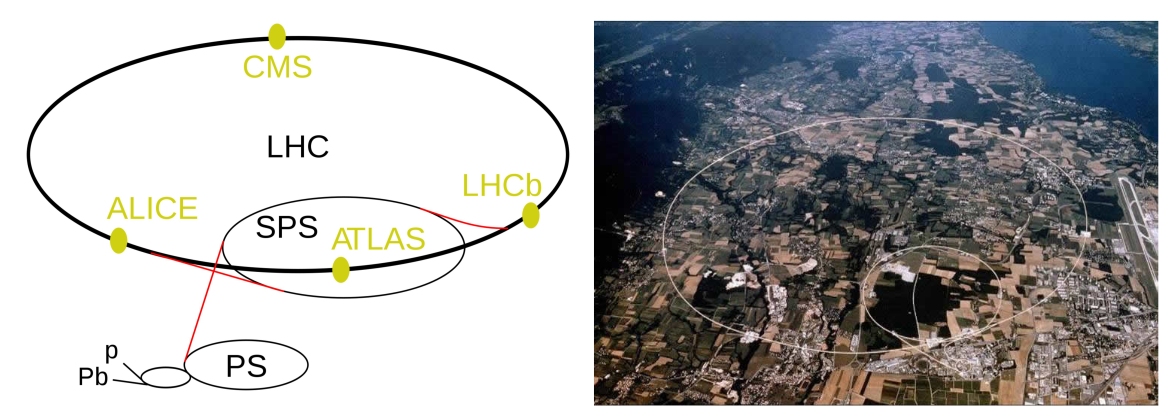
\includegraphics[scale=0.3]{LHC.png}
    \caption{Left: A diagram of the LHC and its rings.\\ Right: An overhead picture of the LHC where you can see Lake Geneva on top of it.}
    \label{fig:fig_3-1}
 \end{figure}

 \begin{figure} %  figure placement: here, top, bottom, or page
    \centering
 %   
\includegraphics[width=\textwidth,height=\textheight,keepaspectratio]{fig_2-1}
    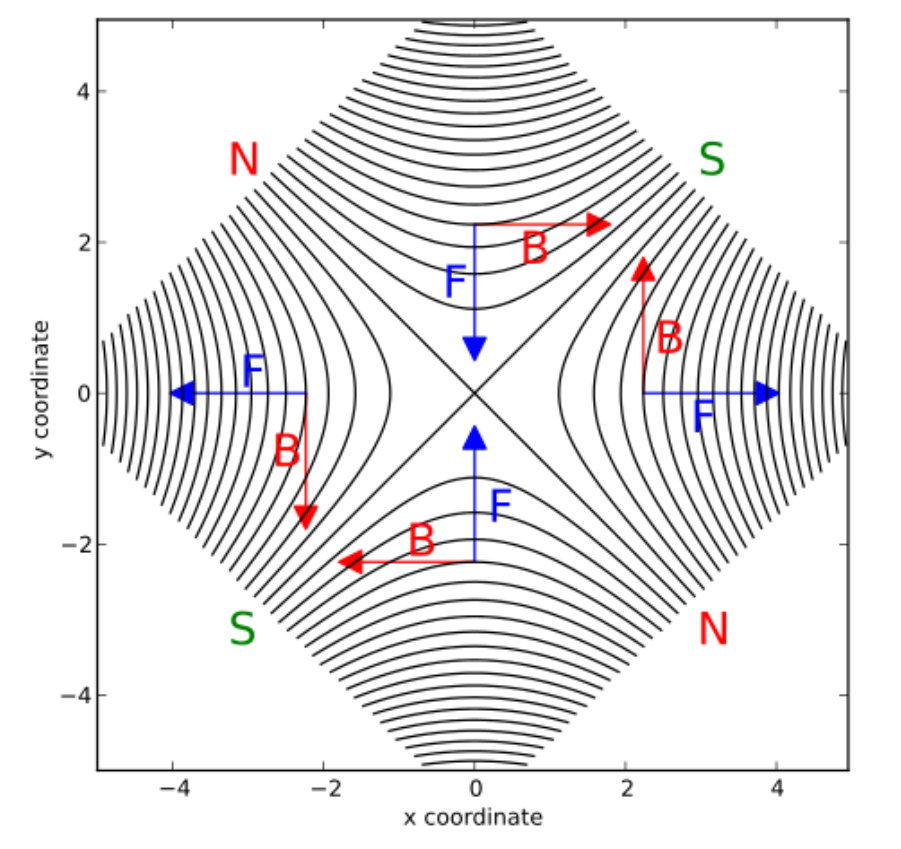
\includegraphics[scale=0.4]{quadrupoleField.png}
    \caption{The quadrupole magnetic field that allows the proton beams to be focused in both horizontal and vertical directions.}
    \label{fig:fig_3-2}
 \end{figure}


\subsection{Proton-Proton Collisions at the LHC}
I previously had said that the proton was made up of a combination of up and down quarks. This is actually an oversimplification of the inside of a proton.
In order for us to understand why one would want to smash protons together we need to get into some of the details about the proton.
While it is true that the proton has two up and one down quark, the interactions between those quarks are dynamic and make up the rest of the picture of the inside of the proton.
There is not actually one gluon per pair of quarks, as one might have thought, but a whole web of gluons that interact with each other and the up and down quarks.
Gluons interacting with each other creates pairs of quarks of all types that then decay back into gluons. 
This is a very important distinction because it powers the modern program of particle physics.
When two protons collide, at the energies of the LHC, we are actually smashing together all of the quarks and gluons currently present in those protons.
In this ``soup'' of interactions, we collectively call the gluons and quarks ``partons''.

The next important question is to ask what was actually collided in a given proton-proton collision.
As previously stated, it is a complicated interaction of quarks and gluons that is not predetermined.
In order to probe this complicated set of interactions, the Parton Distribution Function\footnote{This is usually abbreviated as PDF.} must be computed. 
Instead of trying to find out collision by collision what has happened, the PDF is computed to create a statistical model that can provide an expectation.
The PDF models are very important for discovering new physics because many predicted new particles happen under only specific interactions.
Therefore, if without knowing what to expect in a given proton-proton collision at a given energy, then one cannot know where to look for any undiscovered particle.
Unfortunately, PDFs are very hard to compute. They are approximated by combining partial combinations with high precision measurements from fixed target colliders in order to approach the true PDF.
Since it is only an approximation, one needs to assign a systematic error to the PDF based on the variance of likely PDFs. 
This will be a theme revisited later in the thesis. In order to make a measurement, it will need to be approximated, and therefore it will be necessary to assign systematic uncertainty.

\section{The Compact Muon Solenoid Detector}
There are 4 detector experiments at the LHC. The Compact Muon Solenoid (CMS), shown in Figure \ref{fig:fig_3-3}, is the detector that took the data we are using to perform this analysis.
While it is quite massive compared to a human, weighing in at 14,000 tons, it is actually smaller than the other detectors.
Once again, a full description of CMS and the work done by over 5000 scientists would take many more pages to write so we will confine our discussion to a small overview just to make sure the main parts of the detector are understood.

\begin{figure} %  figure placement: here, top, bottom, or page
   \centering
%   
\includegraphics[width=\textwidth,height=\textheight,keepaspectratio]{fig_2-1}
   \includegraphics[scale=0.043]{cmsDetector.png}
   \caption{A detailed cross section of the CMS detector.}
   \label{fig:fig_3-3}
\end{figure}

\clearpage
\subsection{Coordinate System}
CMS is essentially a large tube where both ends are covered. In order to describe this geometry, we use a modified spherical coordinate system.
The angles used are $\eta$ and $\phi$ where $\phi$ creates the circular component of the cylinder, and will always be perpendicular to the beam.
$\eta$ is defined as:
\begin{equation}
   \eta = -ln  \left( tan \frac{\theta}{2} \right)
\end{equation} 
and is also known as the \textit{pseudorapidity}. Here $\theta$ is the usual angle from spherical coordinates. 
In these coordinates, $\eta = 0$ points straight out of the detector and $\eta = \inf$ points directly along the beampipe.
One reason to use these coordinates is that $\eta$ is approximately Lorentz invariant \footnote{This means that it does not change depending on the reference frame in which we are looking at the interaction. It is always good to work with Lorentz invariant quantities in physics.}
This is necessary because while the protons themselves will have the same energy and likely be symmetric, there is no such guarantee with the partons. 
When we are talking about particles in the detector, we usually talk about them in terms of three values: radial angle $\phi$, pseudorapidity $\eta$, and transverse momentum $p_T$.
If one is interested in returning to Cartesian coordinates, which we are almost never going to do, the following equations will accomplish this task:
\begin{equation}
   p_x = p_T cos(\theta) \quad p_y = p_T sin(\theta) \quad p_z = p_T cosh(\eta)
\end{equation}

\subsection{The Tracker}
The first layer that a particle shot out of a proton-proton collision would encounter is called the Silicon Tracker. 
This layer is directly on the beampipe and consists of 13 individual layers surrounding the beampipe and 14 layers in the endcaps.
These individual layers are bunched together and the first 4 are made up of 66 million silicon pixels that are 100 x 150 $\mu m$ in area. The rest of the layers are made of strip pixels which are longer than the first set.
All of this makes for 200 square meters of silicon that will measure the momentum of any charged particle moving through it.

A magnetic field is applied throughout the silicon tracker which causes any charged particle to curve.
We can then measure the momentum because it will deposit charge on the way through each layer of the silicon tracker. 
With these ``hits'', we can reconstruct the path and therefore the curvature which will allow us to calculate its charge and energy.
The reconstruction of the hits in the silicon tracker of individual particles are called tracks and are determined to an accuracy of about 10 $\mu m$.
The silicon tracker, unlike the rest of the detector, does not try to stop any particle, just measure it as it is shooting towards the calorimeters

\subsection{The Calorimeters}

Recall that different types of particles will interact in different ways, most notably, some particles are much heavier than others.
The first layer outside of the tracker is called the Electromagnetic Calorimeter (ECAL) and is designed to allow photons and electrons to deposit their energy in this layer. 
Heavier particles, namely the hadrons, will move through this part of the detector and not deposit any energy. The Hadron Calorimeter (HCAL) is the next layer and is designed to stop the heavier particles.

The ECAL is composed of around 80,000 lead-tungstate ($PbWO_4$) crystals that are a type of scintillator.
Scintillators emit light when a particle deposits energy into it. So the ECAL will scintillate when light charged particles impact with the crystals.
Since photons have no mass, you might wonder how they interact. The photon can either produce a pair of electrons that will interact with the scintillator or interact with an electron in the crystal itself.
Since these photons and electrons are typically very energetic, they can interact multiple times and create cascades of light or ``showers'' as byproducts of the initial interaction.
The light that is produced is directly proportional to the energy of the initial particle and therefore gives us the missing piece of the puzzle to identify photons and electrons in the detector.

The HCAL is setup a little differently. Instead of crystal scintillators, it has plastic ones that are layered in between brass plates.
The heavy particle will be stopped by the brass plate. This will cause a shower of secondary particles that are measured by the scintillators.
Knowing what kinds of particles can decay to what final states, through the careful study of the rules of the SM, it is then possible to reconstruct what particle hit the HCAL.
It should be noted that the HCAL is the only part of the detector that can stop neutrally charged particles, like neutrons and some mesons, so it is very important for the CMS research program.

\subsection{The Solenoid}

All of the previous layers are contained in a large cylindrical electromagnet called the solenoid.
This electromagnet provides a very large magnetic field (3.8 Tesla \footnote{A normal bar magnet is measured in millitesla!}) which causes electrically charged particles to bend due to the lorentz force.
This effect is dependant on the energy of the particle so the information can be combined with the silicon tracker to measure the momentum of the particle.
This magnetic field is strong enough to shift the alignment of the whole detector and this effect has to be accounted for.
The last layer before the solenoid, the HCAL, uses brass specifically because it is non magnetic. 

\subsection{The Muon Chambers}

After the solenoid there is one final set of detectors. The issue these solve is that muons\footnote{Muons are always problematic!} are too heavy to be stopped by the ECAL and not heavy enough to be stopped by the HCAL.
Muons will go through both and then be stopped by the aptly named Muon Chambers. There are three kinds of muon chambers; drift tubes, cathode strip chambers, and resistive plate chambers, all of which work under the principle that as a muons traverses them, an electron is knocked off of gas atoms.
The amount of electrons that a muon displaces is proportional to its energy and so we can measure the energy of muons with the muons chambers.
Another important thing to note is that, due to the many layers of this detector and the specialities of each type, the muons chamber system is very good at reducing and filtering background noise.


\section{Jets}

In describing the strong force, I mentioned that colored particles cannot exist outside of a color singlet state, meaning they must be in pairs.
In proton-proton collisions, bare quarks (quarks NOT in a color singlet state) can be produced. As soon as they are produced they begin the process of hadronization: creating new particles out of the vacuum until no bare quarks remain.
Gluons may also be created in proton-proton collisions but they will decay to quarks which must then undergo hadronization.
Due to hadronization, the LHC is not able to see individual quarks and gluons. All that can be seen is the shower of hadronized quarks in the direction that the quark or gluon was moving.
The showers are called ``Jets''. The jets are composed of constituent particles, which may in turn decay and leave traces in parts of the detector. These secondary particles are also considered constituents of the jet.
The only particles that are not able to be counted as constituents are neutrinos as their energy is lost in the detector. 

\subsection{The Particle Flow Algorithm}
All of the information from the subdetectors is analyzed by the \textit{Particle Flow Algorithm}. This algorithm allows us to reconstruct jets with a high degree of precision.
It start in the silicon tracker. This subdetector is the crucial part of the algorithm because it makes the initial measurement. If it misses a charged particle, it will bias any reconstruction of that particle. 
Accordingly, great care has been taken to achieve high efficiencies. An iterative tracking strategy allows for extremely high efficiencies in the first pass with softer acceptance for follow up iterations. 
Next, a clustering algorithm is used in the calorimeters to detect and measure the energy of stable neutral particles, separate neutral from charged particles, reconstruct charged electromagnetically charged particles, and aid in the energy measurements for low-quality tracks.
Finally, a link algorithm links the track detected in the silicon tracker with the appropriate clustering in the calorimeter if the extrapolation of the track fits within a given cluster's boundaries.
This is a quick overview of the algorithm because, as is usual in most high energy physics topics, a full description would be beyond the scope of this thesis.

\subsection{Anti-KT Algorithm}

Since most of the events at CMS will generate more than one quarks or gluon, a number of algorithms exists to correctly ``cluster'' the constituents into the right jet.
The one we use and will describe is called the \textit{Anti-$K_t$} Algorithm. The algorithm is an iterative algorithm and runs in the following way.
First, every PF (Particle Flow) candidate is compared against every other candidate with a distance like parameter, $d_{ij}$, given as:
\begin{equation}
   d_{ij} = min(\frac{1}{p_{T,i}^2},\frac{1}{p_{T,j}^2}) \frac{(y_i - y_j)^2+(\phi_i - \phi_j)^2}{R^2}
\end{equation}
where $R$ is a predetermined distance parameter that sets the size of the jet. The two closest constituents are paired and become a new constituent.
This process continues, generating new ``pseudo-jets'', until the distance of the pseudo-jet from the beam is $1/p_T^2$ of the pseudo-jet. It is then removed from consideration and the process starts again with the remaining constituents until none remain.

This algorithm creates what are called ``conical'' jets, with smooth, rounded edges\footnote{This does not always happen, especially with jets that are very close to each other.}.
We call these jets AKR jets, where we use the actual value of R in the naming. Accordingly, an AK8 jet is a jet constructed with the R value of 0.8.
We use AK8 jets and AK4 jets in this analysis. For smaller particles, jets are useful for reconstructing kinematic properties. 
For the larger particles, heavy bosons and quarks, AKR jets can reconstruct the particle with a good degree of accuracy. A simplistic rule with this algorithm is the R value the larger the particle that can be reconstructed.

\section{The Trigger\label{s:trigger}}

Each crossing of proton-proton bunches generates about 1 Megabyte of data. At the rate of 1 crossing every 25 nanoseconds, or 40 Megahertz, no modern computing system can actually keep up with this rate of data generation. 
This means the majority of the data is thrown out. The system responsible for filtering through all of the data is called the ``trigger''.
The trigger operates in two stages, the Level 1 trigger and the High Level trigger. 

The level 1 trigger is a hardware trigger. Output from the detector is stored in a buffer and then it is analyzed by custom circuits. 
These circuits look for ``interesting'' physics, such as especially large deposits in the calorimeters. 
This stage is very useful because it allows the rejection of all but about 0.1 \% of all events.
The rate of release to the next stage is around 50 kilohertz.

The High Level trigger takes the output from level 1 and analyzes the data further in order to find interesting events.
At this level, there are many available triggers depending on what kind of event you are looking for. The selections are mostly kinematic differences.
This is one of the first steps in conducting an analysis. One studies the available triggers in order to understand how your kinematic selections will effect the trigger efficiency.

For our analysis, the trigger algorithm used places requirements on the scalar sum of the jet transverse energy, $H_t$, jet $p_T$, and the jet groomed mass. 
We compensate for the difference in the trigger response between data and simulation by applying a trigger scale factor, defined as the ratio of trigger efficiency in data divided by the trigger efficiency in qcd, to simulated events. 
The trigger efficiency is defined as the ratio of the number of events passing the combined triggers and a pre-trigger to the number that pass the pre-trigger and is parameterized as a function of our measurement variable. 
The trigger efficiency in simulation is modeled by weighting simulated events by this data-derived trigger efficiency. 
We select events from the 2016 dataset that pass the \texttt{HLT\_HT650} trigger, the \texttt{HLT\_PFHT800} trigger or the \texttt{HLT\_PFHT900} trigger, and the \texttt{HLT\_AK8PFJet360\_TrimMass30} trigger. 
For 2017 and 2018, we select events that pass the \texttt{HLT\_PFHT1050} and the \texttt{HLT\_AK8PFJet400\_TrimMass30} trigger are used to select events for the trigger efficiency measurement. 
The pre-trigger for 2016, 2017, and 2018 is the \texttt{HLT\_Jet260} trigger.
Trigger scale factors are measured as a function of the reduced mass, which will be further discussed in Chapter 5. 
After passing the trigger, the events are required to have at least one reconstructed pp collision vertex satisfying the following criteria:
\begin{itemize}{}
\item Vertex number of degrees of freedom $> 4$;
\item Absolute displacement from the beamspot position along the $z$ direction $< 4$ cm;
\item Absolute displacement from the beamspot position along the transverse direction $< 2$ cm.
\end{itemize}

Trigger scale factors are shown here in Figures \ref{fig:fig_3-4}, \ref{fig:fig_3-5}, \ref{fig:fig_3-6}.
\begin{figure}[!htb]
	\centering
	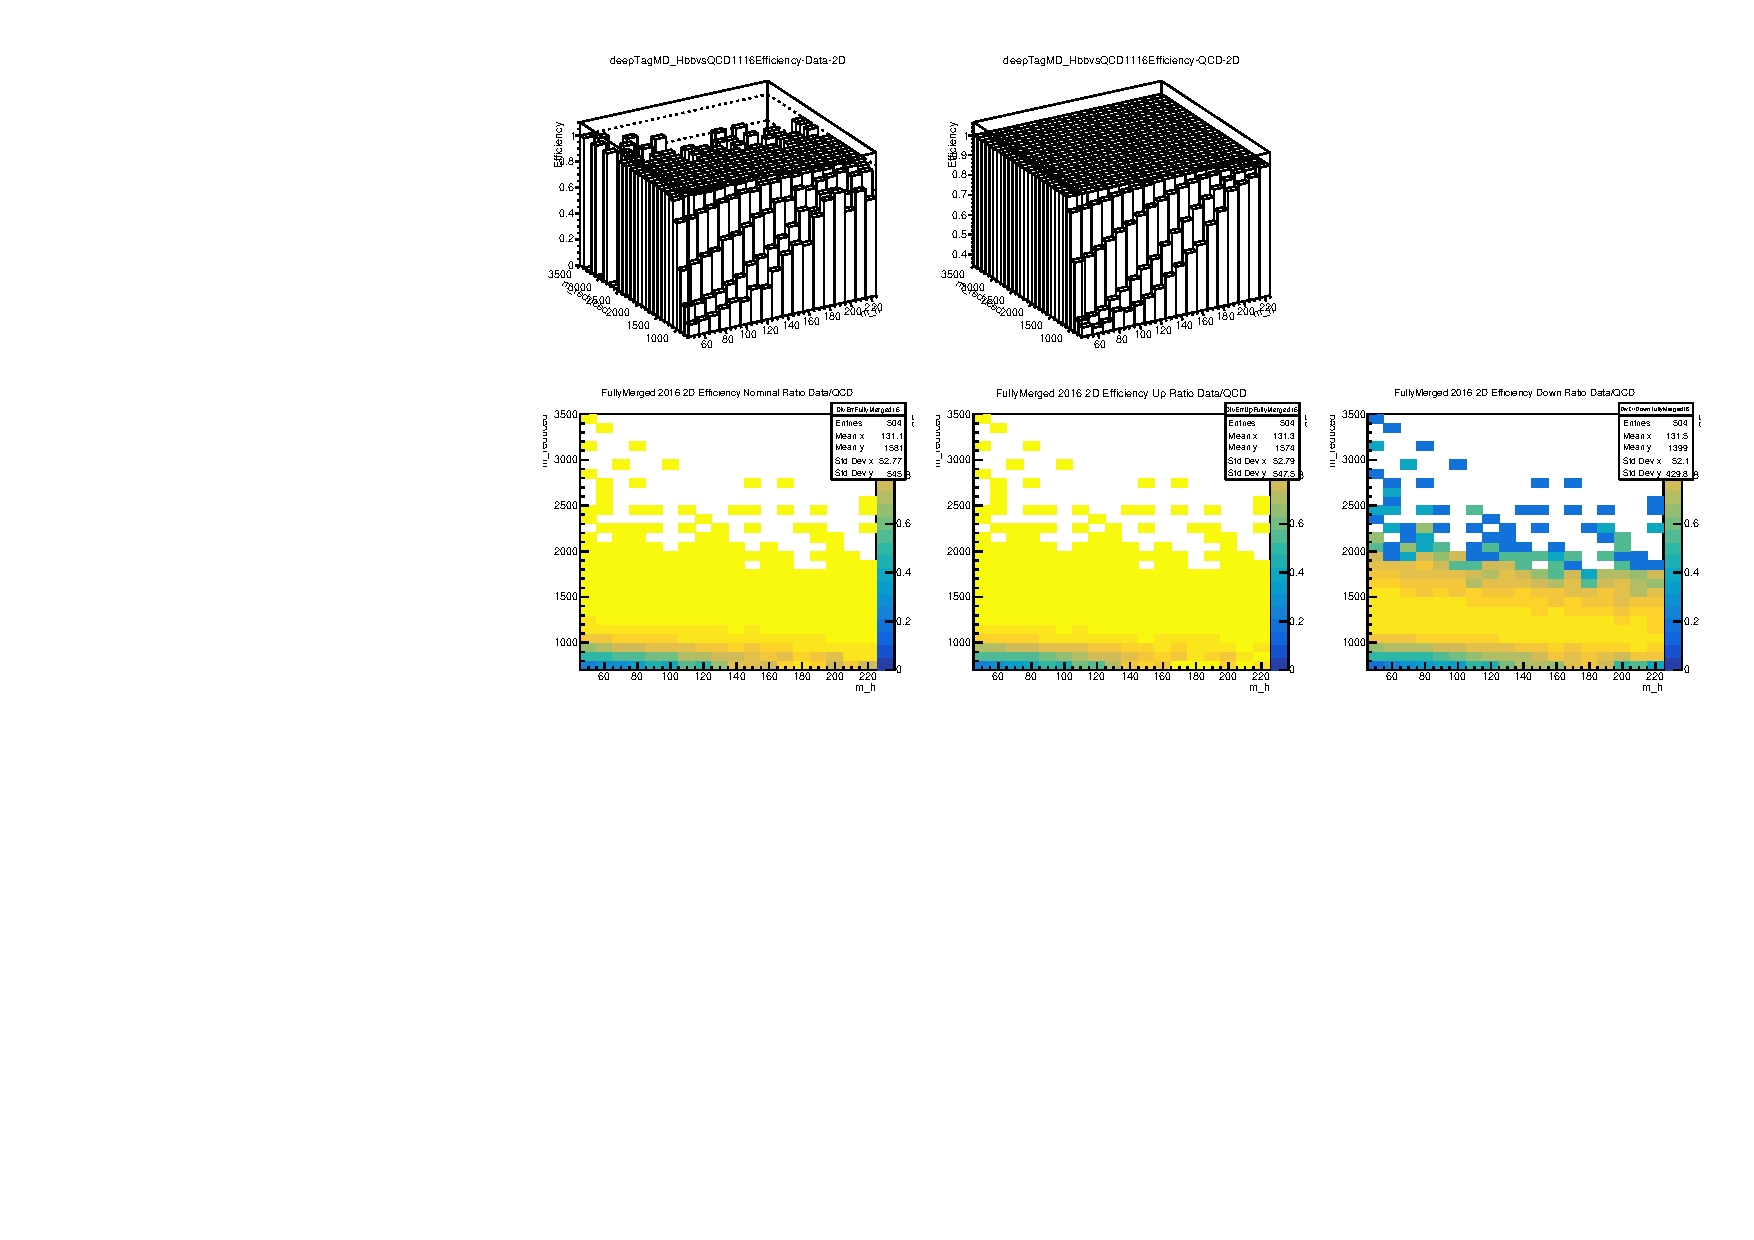
\includegraphics[width=1.0\textwidth]{Figures/2016triggerMaps.pdf}
	\caption{2016 2-Dimensional Trigger Efficiency Scale Factor.}
	\label{fig:fig_3-4}
\end{figure}
\begin{figure}[!htb]
	\centering
	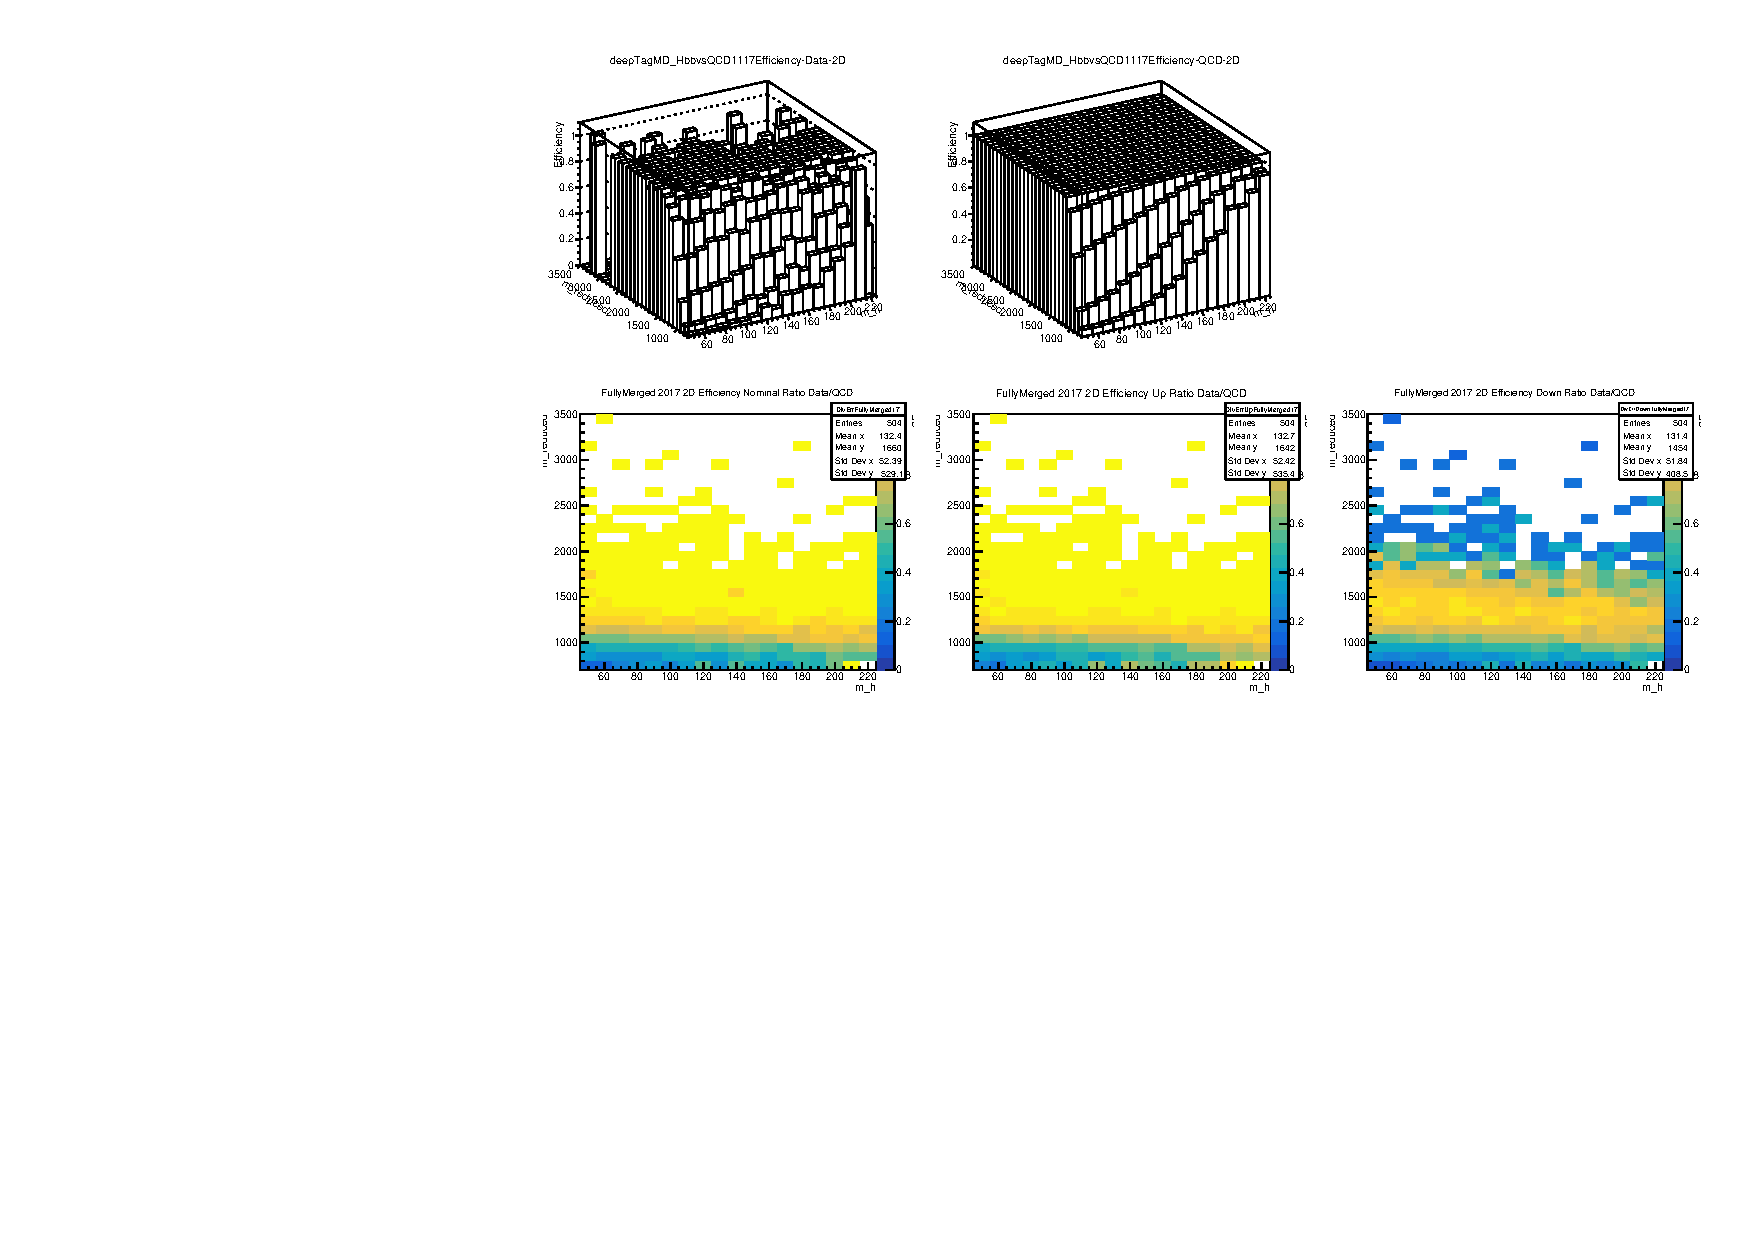
\includegraphics[width=1.0\textwidth]{Figures/2017triggerMaps.pdf}
	\caption{2017 2-Dimensional Trigger Efficiency Scale Factor.}
	\label{fig:fig_3-5}
\end{figure}
\begin{figure}[!htb]
	\centering
	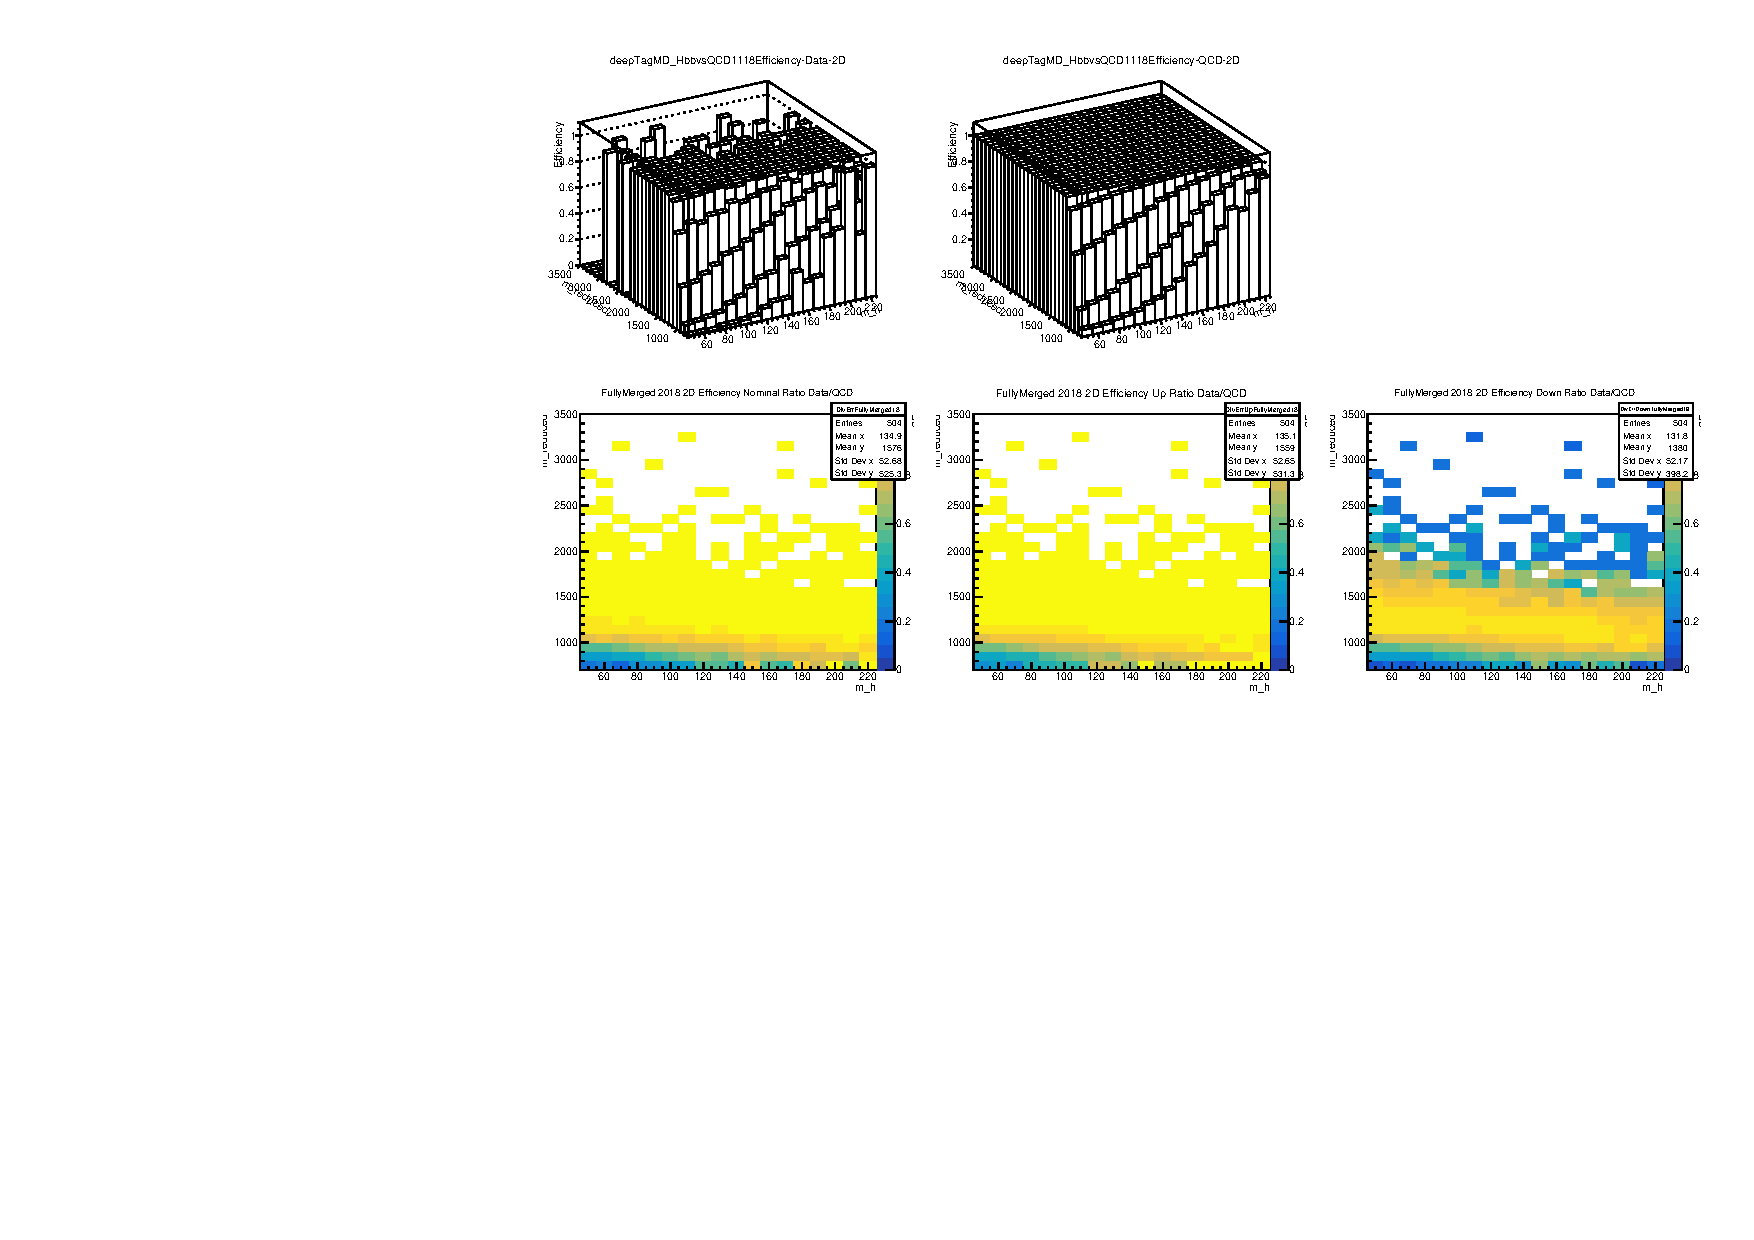
\includegraphics[width=1.0\textwidth]{Figures/2018triggerMaps.pdf}
	\caption{2018 2-Dimensional Trigger Efficiency Scale Factor.}
	\label{fig:fig_3-6}
\end{figure}
\clearpage

\section{Pileup}

Proton-proton collision events are ideally one proton colliding into one proton. 
However, since they are collided in bunches of protons, this is not the reality of what happens.
Events may consist of up to 40 such proton-proton collisions. Therefore, it is necessary to define the primary vertex.
A vertex is a point along the beam from which some number of particle flow candidates originate from.
The primary vertex is selected as the vertex with the highest value for the sum of the square of the transverse momenta of tracks and candidates associated.

Pileup is when the jets coming from the primary vertex contain particle flow candidates that actually originate from a different vertex.
This effect ends up smearing the actual measurement of jet mass and momentum and so we must take this effect into account.
The choice of the AK8 and AK4 clustering algorithm is partly motivated by the fact that the Anti-$k_T$ algorithm resists these effects better than other jet clustering algorithms.

\section{Samples}

\subsection{Data samples\label{ss:DataSamples}}

The analysis is performed using $\Pp\Pp$ interactions collected with the CMS detector at $\sqrt{s}=13~\TeV$. The data correspond an integrated luminosity of \intLumi, as measured using the golden JSON files as follows:
\begin{itemize}
\item 2016: {\footnotesize \href{https://cms-service-dqm.web.cern.ch/cms-service-dqm/CAF/certification/Collisions16/13TeV/ReReco/Final/Cert_271036-284044_13TeV_23Sep2016ReReco_Collisions16_JSON.txt}{Cert\_271036-284044\_13TeV\_23Sep2016ReReco\_Collisions16\_JSON.txt}}
\item 2017: {\footnotesize \href{https://cms-service-dqm.web.cern.ch/cms-service-dqm/CAF/certification/Collisions17/13TeV/ReReco/Cert_294927-306462_13TeV_EOY2017ReReco_Collisions17_JSON.txt}{Cert\_294927-306462\_13TeV\_EOY2017ReReco\_Collisions17\_JSON.txt}}
\item 2018: {\scriptsize \href{https://cms-service-dqm.web.cern.ch/cms-service-dqm/CAF/certification/Collisions18/13TeV/ReReco/Cert_314472-325175_13TeV_17SeptEarlyReReco2018ABC_PromptEraD_Collisions18_JSON.txt}{Cert\_314472-325175\_13TeV\_17SeptEarlyReReco2018ABC\_PromptEraD\_Collisions18\_JSON.txt}}
\end{itemize}
The data samples are summarized in Table \ref{tab:data}. Unless otherwise noted, all data, QCD, \ttbar, and signal samples are processed from nanoAOD version 7. 

\begin{table}[htb]\footnotesize
  \begin{center}
    % \topcaption{List of primary datasets for the \Pp\Pp\,collisions at $\sqrt{s} = 13~\TeV$ and their corresponding integrated luminosities. The golden JSON file \href{https://cms-service-dqm.web.cern.ch/cms-service-dqm/CAF/certification/Collisions16/13TeV/ReReco/Final/Cert_271036-284044_13TeV_23Sep2016ReReco_Collisions16_JSON.txt}{Cert\_271036-284044\_13TeV\_23Sep2016ReReco\_Collisions16\_JSON.txt} was used.}
    \caption{List of primary datasets for the \Pp\Pp\,collisions at $\sqrt{s} = 13~\TeV$ and their corresponding integrated luminosities. The golden JSON files were used are given above.} %\href{https://cms-service-dqm.web.cern.ch/cms-service-dqm/CAF/certification/Collisions16/13TeV/ReReco/Final/Cert_271036-284044_13TeV_23Sep2016ReReco_Collisions16_JSON.txt}{Cert\_271036-284044\_13TeV\_23Sep2016ReReco\_Collisions16\_JSON.txt} was used.}

    \begin{tabular}{l|c|c}
      \hline
      \hline
      Dataset & Processing & Int. lumi. (fb$^{-1}$) \\
      \hline
      JetHT/Run2016B2   & 01June2019 & 5.746  \\
      JetHT/Run2016C   & 01June2019 & 2.573  \\
      JetHT/Run2016D   & 01June2019 & 4.242  \\
      JetHT/Run2016E   & 01June2019 & 4.025  \\
      JetHT/Run2016F   & 01June2019 & 3.105  \\
      JetHT/Run2016G   & 01June2019 & 7.576  \\ 
      JetHT/Run2016H   & 01June2019 & 8.651 \\ 
      JetHT/Run2017B   & 01June2019 & 4.794  \\
      JetHT/Run2017C   & 01June2019 & 9.631  \\
      JetHT/Run2017D   & 01June2019 & 4.248  \\
      JetHT/Run2017E   & 01June2019 & 9.314  \\
      JetHT/Run2017F   & 01June2019 & 13.53  \\
      JetHT/Run2018A   & 01June2019 & 14.03  \\
      JetHT/Run2018B   & 01June2019 & 7.061  \\
      JetHT/Run2018C1   & 01June2019 & 6.895  \\
      % JetHT/Run2018C2   & 01June2019 & 0.305  \\
      JetHT/Run2018D   & 01June2019 & 31.71  \\
      \hline
      Total & & \intLumi \\ 
      \hline
      \hline  
    \end{tabular}  
    \label{tab:data}
  \end{center}
\end{table}

\subsection{MC simulation\label{ss:MCSimulation}}
The MC samples used for this analysis includes spin-2 bulk graviton and spin-0 radion resonances, as given in Table~\ref{tab:signal_MC}, as well as multijet and \ttbar MC, as given in Table~\ref{tab:bkg_MC}. 
We use the puWeightProducer module in ``auto'' mode form the NanoAOD-tools to perform the calculation of the weight.
\begin{table}[htb]\scriptsize
  \begin{center}
    \caption{List of background Monte Carlo samples used. The two \ttjets samples correspond to two different productions with the same generator parameters, but the latter with a much higher statistics. The cross sections $\sigma$ and number of events generated are also given. The cross sections for the QCD processes are at LO. The other SM background cross sections are taken from Ref.~\cite{SMXsecTWiki13TeV}.}    
    \begin{tabular}{l|c|c}
      \hline
      \hline
      \multicolumn{3}{c}{Background} \\ \cline{1-3}
      2016 Process & $\sigma$ (pb) & size \\
      \hline
      % {QCD\_HT-100to200}   & $2.785\times 10^7 $ (LO) & 81,906,377 \\
      % {QCD\_HT-200to300}   & $1.717\times 10^6 $ (LO) & 18,752,566 \\
      % {QCD\_HT-300to500}   & $3.513\times 10^5 $ (LO) & 20,312,907 \\
      % {QCD\_HT-500to700}   & $3.163\times 10^4 $ (LO) & 19,755,616 \\
      {QCD\_HT700to1000\_TuneCUETP8M1\_13TeV-madgraphMLM-pythia8}  & $6.831\times 10^3$  (LO) & 15,629,253 \\
      {QCD\_HT1000to1500\_TuneCUETP8M1\_13TeV-madgraphMLM-pythia8} & $1.207\times 10^3$  (LO) & 48,50,746  \\
      {QCD\_HT1500to2000\_TuneCUETP8M1\_13TeV-madgraphMLM-pythia8} & $119.9 $            (LO) & 3,970,819  \\
      {QCD\_HT2000toInf\_TuneCUETP8M1\_13TeV-madgraphMLM-pythia8}  & $25.24 $            (LO) & 1,991,645  \\
      {QCD\_HT700to1000\_TuneCUETP8M1\_13TeV-madgraphMLM-pythia8\_ext1-v1}  & $6.831\times 10^3$  (LO) & 21,604,533 \\
      {QCD\_HT1000to1500\_TuneCUETP8M1\_13TeV-madgraphMLM-pythia8\_ext1-v1} & $1.207\times 10^3$  (LO) & 10,360,193  \\
      {QCD\_HT1500to2000\_TuneCUETP8M1\_13TeV-madgraphMLM-pythia8\_ext1-v1} & $119.9 $            (LO) & 7,868,538   \\
      {QCD\_HT2000toInf\_TuneCUETP8M1\_13TeV-madgraphMLM-pythia8\_ext1-v1}  & $25.24 $            (LO) & 3,812,534  \\
      \hline
      {TT\_TuneCUETP8M2T4\_13TeV-powheg-pythia8} & $831.76$ (NNLO) & 76,367,863 \\
      % {TT\_TuneCUETP8M2T4\_13TeV-powheg-pythia8} & $831.76$ (NNLO) & 96,834,559 \\
      \hline
      \hline

      2017 Process & $\sigma$ (pb) & size \\
      \hline

      {QCD\_HT700to1000\_TuneCP5\_13TeV-madgraphMLM-pythia8}  & $6.831\times 10^3$  (LO) & 47,610,552 \\
      {QCD\_HT1000to1500\_TuneCP5\_13TeV-madgraphMLM-pythia8} & $1.207\times 10^3$  (LO) & 16,595,628  \\
      {QCD\_HT1500to2000\_TuneCP5\_13TeV-madgraphMLM-pythia8} & $119.9 $            (LO) & 11,634,434  \\
      {QCD\_HT2000toInf\_TuneCP5\_13TeV-madgraphMLM-pythia8}  & $25.24 $            (LO) & 5,941,306  \\
      \hline
      {TTToHadronic\_TuneCP5\_PSweights\_13TeV-powheg-pythia8} & $377.96$ (NNLO) & 130,091,218 \\
      {TTToSemiLeptonic\_TuneCP5\_PSweights\_13TeV-powheg-pythia8} & $365.34$ (NNLO) & 109,663,792 \\
      \hline
      \hline

      2018 Process & $\sigma$ (pb) & size \\
      \hline

      {QCD\_HT700to1000\_TuneCP5\_13TeV-madgraphMLM-pythia8}  & $6.831\times 10^3$  (LO) & 48,158,738 \\
      {QCD\_HT1000to1500\_TuneCP5\_13TeV-madgraphMLM-pythia8} & $1.207\times 10^3$  (LO) & 15,466,225  \\
      {QCD\_HT1500to2000\_TuneCP5\_13TeV-madgraphMLM-pythia8} & $119.9 $            (LO) & 10,955,087  \\
      {QCD\_HT2000toInf\_TuneCP5\_13TeV-madgraphMLM-pythia8}  & $25.24 $            (LO) & 5,475,677  \\
      \hline
      {TTToHadronic\_TuneCP5\_13TeV-powheg-pythia8} & $377.96$ (NNLO) & 128,640,000 \\
      {TTToSemiLeptonic\_TuneCP5\_13TeV-powheg-pythia8} & $365.34$ (NNLO) & 100,790,000 \\
      \hline
      \hline
    \end{tabular}
    \label{tab:bkg_MC}
  \end{center}
\end{table}

\subsection{Theory predictions\label{ss:SignalXsec}}

\begin{table}[h]
  \begin{center}
    \caption{\small NLO Bulk graviton and radion cross sections cross sections times the decay rate for the samples that are used to set a limit (lower mass samples were studied but the analysis is not sensitive below 750 GeV). 
    The bulk graviton production cross sections are evaluated for $k/\overline{\Mpl} = 0.1$~\cite{WED_BG_13TeV} then multiplied by 25 to get the values for $k/\overline{\Mpl} = 0.5$, and the radion cross sections for $\Lambda_{\rm R} = 3\TeV$ and $kl = 35$~\cite{WED_radion_13TeV}. 
    The bulk graviton and radion to $\PH\PH$ decay branching fractions are taken from Refs.~\cite{WED_BGHHDecay_13TeV} and ~\cite{WED_radionHHDecay_13TeV}, respectively. All cross sections listed in Ref.~\cite{KKGraviton_Bulk_github}.}
    \begin{tabular}{l|ccccc} 
      \hline
      \hline
      $\mx$ (GeV) & \multicolumn{2}{c}{Bulk graviton (fb)} & \multicolumn{2}{c}{Radion (fb)} \\ \cline{2-5}
      & $\sigma(\Pp\Pp \to X)$ & $\sigma(\Pp\Pp \to X \to \HH )$ & $\sigma(\Pp\Pp \to X)$ & $\sigma(\Pp\Pp \to X \to \HH )$ \\
      \hline
%      500   &   --      &   --   \\
%      550   &   --      &   --   \\
%      600   &   --      &   --   \\
%      650   &   --      &   --   \\
      1000  & 141.65     & 13.97   & 261.89 & 62.057 \\
      1500  & 14.325     & 1.425    & 54.428 & 12.897 \\
      2000  & 2.265  & 0.22575  & 14.293 & 3.3868 \\
      2500  & 0.4675  & 0.04625  & 4.3017 & 1.0193 \\
      3000  & 0.11025  & 0.0110  & 1.3843 & 0.3280 \\
      %3500  & 1.15E-03  & 1.15E-04 \\ %& 0.4700 & 0.1114 \\
      %4500  & 8.93E-05  & 8.91E-06 \\ %& 5.34E-02 & 1.26E-02 \\
      \hline
      \hline
    \end{tabular}
    \label{tab:signal_MC}
  \end{center}
\end{table}

The NLO bulk graviton and radion cross sections are provided in Table ~\ref{tab:signal_MC} for the mass points used in the analysis. Lower mass points were considered but the analysis is not sensitive below 750 GeV, where the trigger efficiency is extremely poor. 
The bulk graviton production cross sections are evaluated for $k/\overline{\Mpl} = 0.1$~\cite{WED_BG_13TeV} then multiplied by 25 to get the values for $k/\overline{\Mpl} = 0.5$, and the radion cross sections for $\Lambda_{\rm R} = 3\TeV$ and $kl = 35$~\cite{WED_radion_13TeV}. 
The bulk graviton and radion to $\PH\PH$ decay branching fractions are taken from Refs.~\cite{WED_BGHHDecay_13TeV} and ~\cite{WED_radionHHDecay_13TeV}, respectively. 
